\documentclass[a4paper,12pt]{article} % добавить leqno в [] для нумерации слева
\usepackage[a4paper,top=1.3cm,bottom=2cm,left=1.5cm,right=1.5cm,marginparwidth=0.75cm]{geometry}
%%% Работа с русским языком
\usepackage{cmap}					% поиск в PDF
\usepackage[warn]{mathtext} 		% русские буквы в фомулах
\usepackage[T2A]{fontenc}			% кодировка
\usepackage[utf8]{inputenc}			% кодировка исходного текста
\usepackage[english,russian]{babel}	% локализация и переносы
\usepackage{physics}
\usepackage{multirow}
\usepackage{siunitx}

%%% Нормальное размещение таблиц (писать [H] в окружении таблицы)
\usepackage{float}
\restylefloat{table}

\usepackage{graphicx}

\usepackage{caption}
\usepackage{subcaption}

\usepackage{wrapfig}
\usepackage{tabularx}

\usepackage{hyperref}
\usepackage[rgb]{xcolor}
\hypersetup{
	colorlinks=true,urlcolor=blue
}

%%% Дополнительная работа с математикой
\usepackage{amsmath,amsfonts,amssymb,amsthm,mathtools} % AMS
\usepackage{icomma} % "Умная" запятая: $0,2$ --- число, $0, 2$ --- перечисление

%% Номера формул
%\mathtoolsset{showonlyrefs=true} % Показывать номера только у тех формул, на которые есть \eqref{} в тексте.

%% Шрифты
\usepackage{euscript}	 % Шрифт Евклид
\usepackage{mathrsfs} % Красивый матшрифт
\usepackage{pgfplots}
\pgfplotsset{compat=1.9}

%% Свои команды
\DeclareMathOperator{\sgn}{\mathop{sgn}}

%% Не нумеровать секциии
\setcounter{secnumdepth}{0}

%% Перенос знаков в формулах (по Львовскому)
\newcommand*{\hm}[1]{#1\nobreak\discretionary{}
	{\hbox{$\mathsurround=0pt #1$}}{}}

\date{\today}

\begin{document}

\begin{titlepage}
	\begin{center}
		{\large МОСКОВСКИЙ ФИЗИКО-ТЕХНИЧЕСКИЙ ИНСТИТУТ (НАЦИОНАЛЬНЫЙ ИССЛЕДОВАТЕЛЬСКИЙ УНИВЕРСИТЕТ)}
	\end{center}
	\begin{center}
		{\large Физтех-школа прикладной математики и информатики}
	\end{center}
	
	
	\vspace{4.5cm}
	{\huge
		\begin{center}
			{\bf Отчёт о выполнении лабораторной работы 5.1}\\
			Измерение коэффициента ослабления потока $\gamma$-лучей в
                веществе и определение их энергии (+дозиметрия)
		\end{center}
	}
	\vspace{1cm}
	\begin{center}
		{\large Соболевский Федор Александрович \\
             Старокожко Иван Георгиевич \\ 
			\vspace{0.2cm}
			Б05-111}
	\end{center}
	\vspace{8cm}
	\begin{center}
		  Декабрь 2023
	\end{center}
\end{titlepage}

\section{Теоретические положения}

Проходя через вещество, пучок $\gamma$-квантов постепенно ослабляется, ослабление происходит по экспоненциальному закону, который может быть записан в двух эквивалентных формах:
\[\begin{array}{l}
I = I_0 e^{-\mu l} ,\\
I = I_0 e^{-\mu' m_l},\\
\end{array}\]
где $I, I_0$ -- интенсивности прошедшего и падающего излучений, $l$ -- длина пути, пройденного пучком $\gamma$-лучей, $m_l$ -- масса пройденного вещества на единицу площади, $\mu$, $\mu'$ -- константы, зависящие от вещества. Ослабление потока $\gamma$-лучей возникает из-за фотоэлектрического поглощения, комптоновского рассеяния и генерации электрон-позитронных пар (при достаточных энергиях).\\
Считая, что опыт поставлен в \textit{хорошей геометрии}, то есть сквозь вещество всегда идёт узкий параллельный пучок, можно считать, что комптоновское рассеяние выводит $\gamma$-кванты из пучка и в итоге меняется количество, но не энергия $\gamma$-квантов. Это означает, что $\mu$ не зависит от $l$. Число выбывших на пути $dl$ из пучка $\gamma$-квантов
\[-dN = \mu N dl,\]
откуда
\[N = N_0 e^{\mu l},\]
или
\begin{equation}
\mu = \dfrac{1}{l} \ln \dfrac{N_0}{N}.
\end{equation}

\section*{Описание установки}
\begin{figure}[h]
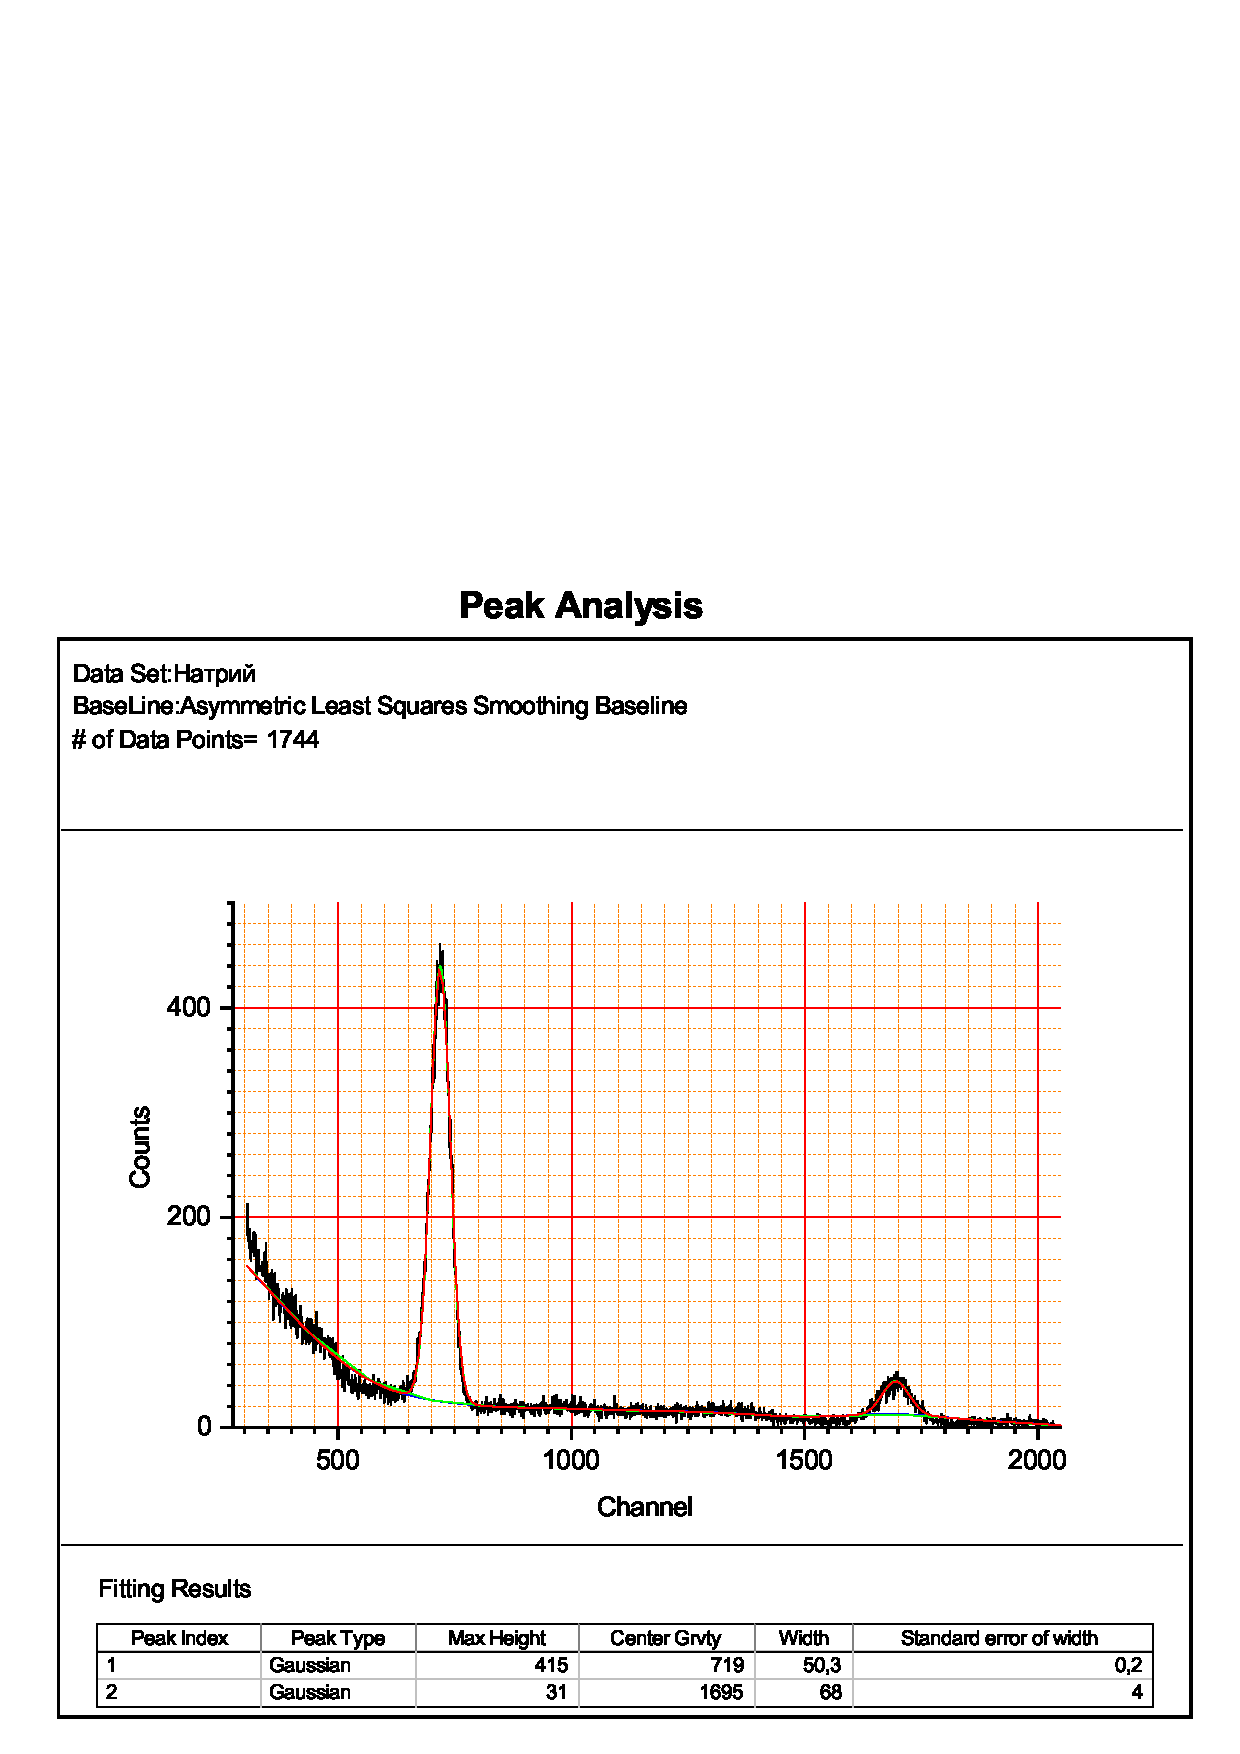
\includegraphics[scale=0.5]{1.png}
\centering
\caption{Схема установки.}
\end{figure}
На Рис. 1 изображена схема установки. Свинцовый коллиматор выделяет узкий почти параллельный пучок $\gamma$-квантов, проходящий через набор поглотителей П и регистрируемый сцинтилляционным счётчиком. Сигналы от счётчика усиливаются и регистрируются пересчётным прибором ПП. Высоковольтный выпрямитель ВВ обеспечивает питание сцинтилляционного счётчика. Чтобы уменьшить влияние плохой геометрии, счётчик расположен на большим расстоянии от источника, поглотители имеют небольшие размеры, а так же устанавливаются на расстоянии друг от друга, чтобы испытавшие комптоновское рассеяние кванты с меньшей вероятностью могли в него вернуться.

\section*{Ход работы, результаты}
\subsection{Измерение фона}
В ходе работы были проведены измерения для определения коэффициента поглащения трех металлов: алюминия (Al), свинца (Pb) и железа (Fe). Промежуток времени, на котором считалось число частиц в каждом наблюдении, сохранялся равным 10с. 

Первое измерение -- фон. Образец был закрыт специальным считом, при этом дачик показал приблизительно постоянные измерения. Результаты представлены в таблице \href{table:back}

\begin{table}[!ht]
    \centering
    \label{table:back}
    \begin{tabular}{|l|l|}
    \hline
        № измерения & $N_0$ \\ \hline
        1 & 336  \\ \hline
        2 & 309  \\ \hline
        3 & 317  \\ \hline
        4 & 329  \\ \hline
        5 & 320  \\ \hline
        6 & 311  \\ \hline
        7 & 318  \\ \hline
        8 & 334  \\ \hline
        9 & 308  \\ \hline
        10 & 331  \\ \hline
        среднее & 321 \\ \hline
        погрешность & $\pm$ 1 \\ \hline
    \end{tabular}
\end{table}

Полученное значение бедут вычитаться из всех последующих измерений, чтобы компенсировать фоновое излучение.

\subsection{Измерение Al}
Первая серия измерений проводилась с образцами из алюминия. Для регулирования толщины поглащающего/рассеивающего слоя использовались металлические бруски толщиной  $l_0 = 2.2\text{см}$. Результаты измерений представлены в таблице 1.

\begin{table}[!ht]
    \centering
    \label{table:Al}
    \caption{Измерения Al}
    \begin{tabular}{|l|l|l|l|l|}
    \hline
        $l_0$ Fe, мм & $\sum l_i$, мм & N & $\frac {l_0}{l}$ & $\ln( \frac {N} {N_0} )$  \\ \hline
        2,2 & 2,2 & 71526 & 1,000 & 1  \\ \hline
        2,2 & 4,4 & 48000 & 0,500 & 0,6696  \\ \hline
        2,2 & 6,6 & 31844 & 0,333 & 0,4427  \\ \hline
        2,2 & 8,8 & 20932 & 0,250 & 0,2895  \\ \hline
        2,2 & 11 & 14321 & 0,200 & 0,1966  \\ \hline
        2,2 & 13,2 & 9675 & 0,167 & 0,1314  \\ \hline
        3,2 & 16,4 & 6815 & 0,195 & 0,0912  \\ \hline
    \end{tabular}
\end{table}

По результатам измерений построим график в логарифмированных координатах. График представлен на рис. \ref{fig:Al_plot}. Из него получаем коэффициент $\mu_{Al} = 1.47 \pm 0.04$, что соответствует энергии $\gamma$-кванта, равной 0.6 МэВ.

\begin{figure}[h]
    \centering
    \includegraphics[width=1\textwidth]{Al_plot.png}
    \caption{График для Al}
    \label{fig:Al_plot}
\end{figure}

\subsection{Измерение Pb}
Вторая серия измерений проводилась аналогично с образцами из свинца. $l_0 = 0.47\text{см}$. Результаты измерений представлены в таблице 2.

\begin{table}[!ht]
    \centering
    \label{table:Pb}
    \caption{Измерения Pb}
    \begin{tabular}{|l|l|l|l|l|}
    \hline
        $l_0$ Fe, мм & $\sum l_i$, мм & N & $\frac {l_0}{l}$ & $\ln( \frac {N} {N_0} )$  \\ \hline
        0,47 & 0,47 & 58182 & 1,000 & 1  \\ \hline
        0,47 & 0,94 & 32415 & 0,500 & 0,5547  \\ \hline
        0,47 & 1,41 & 18851 & 0,333 & 0,3202  \\ \hline
        0,47 & 1,88 & 11189 & 0,250 & 0,1878  \\ \hline
        0,47 & 2,35 & 6628 & 0,200 & 0,1090  \\ \hline
        0,47 & 2,82 & 4064 & 0,167 & 0,0647  \\ \hline
    \end{tabular}
\end{table}

По результатам измерений построим график в логарифмированных координатах. График представлен на рис. \ref{fig:Pb_plot}. Из него получаем коэффициент $\mu_{Pb} = 0.249 \pm 0.01$, что соответствует энергии $\gamma$-кванта, равной 0.6 МэВ.

\begin{figure}[h]
    \centering
    \includegraphics[width=1\textwidth]{Pb_plot.png}
    \caption{График для Pb}
    \label{fig:Pb_plot}
\end{figure}

\subsection{Измерение Fe}
Третья серия измерений проводилась с образцами из железа. $l_0 = 1.01\text{см}$. Результаты измерений представлены в таблице 3.

\begin{table}[!ht]
    \centering
    \label{table:Fe}
    \caption{Измерения Fe}
    \begin{tabular}{|l|l|l|l|l|}
    \hline
        $l_0$ Fe, мм & $\sum l_i$, мм & N & $\frac {l_0}{l}$ & $\ln( \frac {N} {N_0} )$  \\ \hline
        1,01 & 1,01 & 60826 & 1,000 & 1  \\ \hline
        1,01 & 2,02 & 34441 & 0,500 & 0,5639  \\ \hline
        1,01 & 3,03 & 19734 & 0,333 & 0,3208  \\ \hline
        1,01 & 4,04 & 11367 & 0,250 & 0,1826  \\ \hline
        1,01 & 5,05 & 6751 & 0,200 & 0,1063  \\ \hline
        1,01 & 6,06 & 4072 & 0,167 & 0,0620  \\ \hline
    \end{tabular}
\end{table}

По результатам измерений построим график в логарифмированных координатах. График представлен на рис. \ref{fig:Fe_plot}. Из него получаем коэффициент $\mu_{Al} = 0.691 \pm 0.01$, что соответствует энергии $\gamma$-кванта, равной 0.5 МэВ.

\begin{figure}[h]
    \centering
    \includegraphics[width=1\textwidth]{Fe_plot.png}
    \caption{График для Fe}
    \label{fig:Fe_plot}
\end{figure}

\newpage
\subsection{Выводы}
В ходе выполнения лабораторной работы были проведены измерения коэффициента ослабления $\mu$ для гамма-квантов при прохождении через различные материалы: алюминий (Al), свинец (Pb) и железо (Fe).

Для алюминия был получен коэффициент ослабления $\mu_{\text{Al}} = 1.47 \pm 0.04$, что соответствует энергии $\gamma$-кванта, равной приблизительно 0.6 МэВ. Для свинца получен коэффициент $\mu_{\text{Pb}} = 0.249 \pm 0.01$, что также соответствует энергии $\gamma$-кванта около 0.6 МэВ. Наконец, для железа получен коэффициент $\mu_{\text{Fe}} = 0.691 \pm 0.01$, что соответствует энергии $\gamma$-кванта около 0.5 МэВ.

В действительности изучаемое излучение испускает $^{137}Cs$ по каналу $\beta^{-}$, что означает табличное значение энергии гамма-кванта в $0.6617МэВ$. Таким образом, отклонение составляет менее 10\%, что достаточно хорошо сходится с теорией.  

Результаты эксперимента согласуются с теорией ослабления гамма-квантов в веществе и позволяют оценить энергии используемых $\gamma$-квантов. Погрешности измерений в пределах указанных значений свидетельствуют о хорошей точности проведенных измерений.

\end{document}